% Source for docs/assets/results-summary.png (README Results chart).
% Rebuild:  xelatex results-bars.tex && magick -density 300 results-bars.pdf \
%           -background '#0d1117' -flatten results-summary.png
% Data = docs/paper/paper.md Fig. 3 (fpga/fpga_cost*.sh + fmax*.sh outputs).
\documentclass[border=14pt]{standalone}
\usepackage{fontspec}
\setmainfont{DejaVu Sans}
\usepackage{tikz}
\definecolor{bg}{HTML}{0d1117}
\definecolor{track}{HTML}{21262d}
\definecolor{trackline}{HTML}{30363d}
\definecolor{bar}{HTML}{4493f8}
\definecolor{fg}{HTML}{e6edf3}
\definecolor{muted}{HTML}{9198a1}
\pagecolor{bg}
\begin{document}
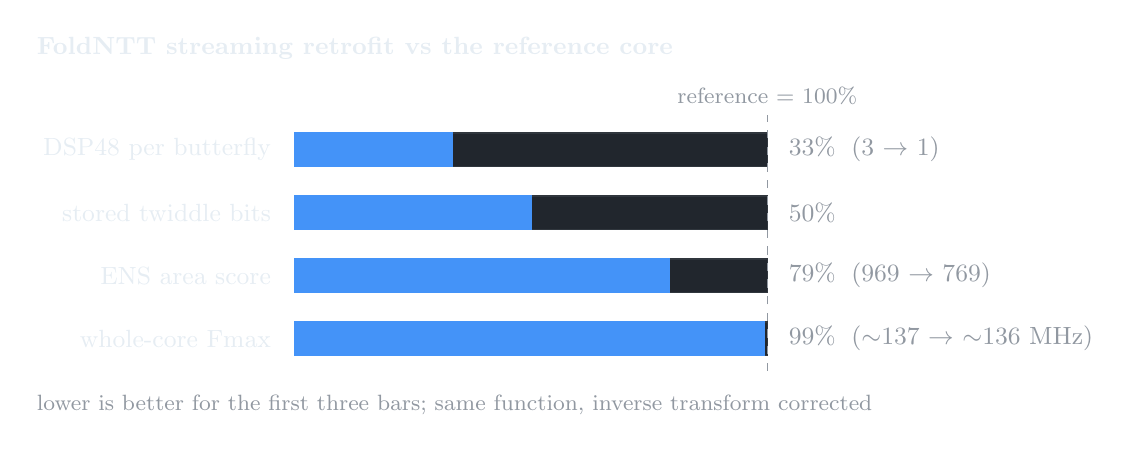
\begin{tikzpicture}[font=\small]
\newcommand{\perfbar}[4]{%
  \draw[fill=track, draw=trackline] (0,#1) rectangle (6.0,#1+0.42);
  \draw[fill=bar, draw=bar] (0,#1) rectangle (#2,#1+0.42);
  \node[anchor=east, text=fg] at (-0.18,#1+0.21) {#3};
  \node[anchor=west, text=muted] at (6.15,#1+0.21) {#4};}
\node[anchor=west, text=fg, font=\small\bfseries] at (-3.4,4.55)
  {FoldNTT streaming retrofit vs the reference core};
\perfbar{3.05}{2.00}{DSP48 per butterfly}{33\%\; (3 $\to$ 1)}
\perfbar{2.25}{3.00}{stored twiddle bits}{50\%}
\perfbar{1.45}{4.76}{ENS area score}{79\%\; (969 $\to$ 769)}
\perfbar{0.65}{5.96}{whole-core Fmax}{99\%\; ($\sim$137 $\to$ $\sim$136 MHz)}
\draw[muted, dashed] (6.0,0.45) -- (6.0,3.70)
  node[above, text=muted, font=\footnotesize] {reference = 100\%};
\node[anchor=west, text=muted, font=\footnotesize] at (-3.4,0.02)
  {lower is better for the first three bars; same function, inverse transform corrected};
\end{tikzpicture}
\end{document}
